\begin{titlepage}
\thispagestyle{empty}
\newgeometry{margin=3cm}
\renewcommand{\arraystretch}{1.5}

\begin{tikzpicture}[remember picture,overlay]
    \node[anchor=north west, inner sep=0pt] 
        at ($(current page.north west)+(3cm, -3cm)$) {
            
\includegraphics[height=2.25cm]{figures/logo/LOGO_SAM}
        };
\end{tikzpicture}

\begin{flushright}
    \LARGE \bfseries
    Anno scolastico \projectyear \\
    Lavoro Professionale Individuale
\end{flushright}

\large
\noindent\begin{tabularx}{\textwidth}{l X}
    \midrule
    Nome Cognome: & \textbf{\name} \\

    \midrule
    Professione: & \textbf{Elettronico} \\

    \midrule
    Titolo del progetto: & \textbf{\project} \\

    \midrule
\end{tabularx}
\vfill

% immagine opizonale
% \includegraphics[\height=]{figures}
\begin{center}
    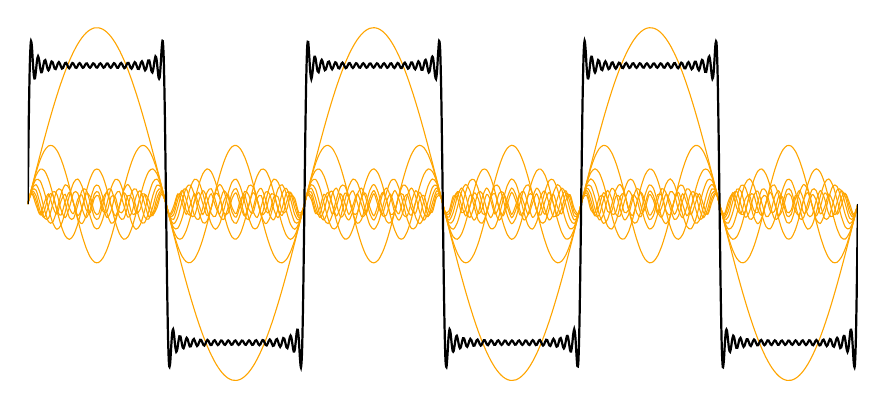
\begin{tikzpicture}[=latex]
		\begin{axis}[
			width = \linewidth,
            height = .5\linewidth,
            axis x line = center,
            axis y line = center,
            xlabel = {\(t\)},
            xlabel style = {right},
            ylabel = {\(y\)},
            ylabel style = {above},
            % axis equal,
            hide axis,
            % xticklabels = \empty,
            % xtick = \empty,
            yticklabels = \empty,
            ytick = \empty,
            domain=0:30
		]
			\def\sumcurve{0}

			\pgfplotsinvokeforeach{1,3,5,...,17}{
                \def\func{sin(deg(#1*x*2*pi/10))/#1/pi}

                \addplot [Orange, smooth, samples=200]{\func};
                \xdef\sumcurve{\sumcurve + \func}
			}

			\pgfplotsinvokeforeach{19,21,23,...,39}{
                \def\func{sin(deg(#1*x*2*pi/10))/#1/pi}

                \xdef\sumcurve{\sumcurve + \func}
			}

			\addplot [Black, thick, smooth, samples=800] {\sumcurve};

            % \draw[black, very thick, ->] (axis cs: 0,0) -- (axis cs: 30,0);
		\end{axis}
	\end{tikzpicture}
\end{center}

\vfill
\noindent\begin{tabularx}{\textwidth}{l X l X}
    \midrule
    Azienda: & \multicolumn{3}{l}{\parbox{5cm}{
        \textbf{CPT Bellinzona} \\
        Centro Professionale Tecnico \\
        Viale S. Franscini 25 \\
        6500 Bellinzona%
    }} \\

    \midrule
    Formazione approfondita: & \multicolumn{3}{l}{\textbf{\specialization}} \\

    \midrule
    Formatore: & \multicolumn{3}{l}{\textbf{\instructor}} \\

    \midrule
    Data d'inizio: & \textbf{\projstart} & Ore a disposizione: & \textbf{\plannedtime}\\

    \midrule
    Data file lavoro: & \textbf{\projend} & Ore effettive: &  \textbf{\actualtime} \\

    % \midrule
    % Data di compilazione & \textbf{\today} \\

    \midrule
\end{tabularx}

\restoregeometry
\end{titlepage}
